% !TEX root = ../../STP_IoTjournal.tex
\subsection{Effects of Disturbance and Scheduled Time of Arrival \label{sec:city_distbEffect}}
In this section, we illustrate how the disturbance bound $d_r$ in \eqref{eq:dyn_i} and the relative $\sta$s of vehicles affect the vehicle trajectories. For this purpose, we simulate the STP algorithm for four additional scenarios:
\begin{itemize}
\item Case-0: $d_r = 6$ m/s, $\sta_i = 0 ~\forall i$ (moderate breeze, high UAV density)
\item Case-1: $d_r = 11$ m/s, $\sta_i = 0 ~\forall i$ (strong breeze, high UAV density)
\item Case-2: $d_r = 6$ m/s, $\sta_i = 5(i-1) ~\forall i$ (moderate breeze, medium UAV density)
\item Case-3: $d_r = 11$ m/s, $\sta_i = 5(i-1) ~\forall i$ (strong breeze, medium UAV density)
\item Case-4: $d_r = 11$ m/s, $\sta_i = 10(i-1) ~\forall i$ (strong breeze, low UAV density)
\end{itemize}
The interpretation $\sta_i = 5(i-1)$ is that the scheduled time of arrival of any two consecutive vehicles is separated by 5 s, which represents a medium vehicle density scenario; a separation of 10 s represents a low vehicle density scenario. $d_r = 6$ m/s and $d_r = 11$ m/s correspond to the moderate breeze and strong breeze respectively on Beaufort wind force scale \cite{Windscale}. 

Intuitively, as $\dstb_r$ increases, it is harder for a vehicle to closely track a particular nominal trajectory, which results in a higher tracking error bound. As mentioned previously, with a $6$ m/s wind speed, the tracking error bound is 5 m; however, with an $11$ m/s wind speed, the tracking error bound becomes 35 m. Thus, the vehicles need to be separated more from each other in space to ensure that they do not enter each other's danger zones. This is also evident from comparing the results corresponding to Case-0 (Fig. \ref{fig:sf_d6sep0}) and Case-1 (Fig. \ref{fig:sf_d11sep0}). As the disturbance magnitude increases from $d_r = 6$ m/s (moderate breeze) to $d_r = 11$ m/s (strong breeze), the vehicles' trajectories get farther apart from each other. Since $\sta$ is same for all vehicles, the vehicles’ trajectories are still predominately \textit{state-separated} trajectories.

We next compare Case-0 and Case-2. The difference between these two cases is that vehicles have a 5 second separation in their schedule times of arrival in Case-2. When vehicles $\veh_i$ and $\veh_{j}$ ($j>i$) have same scheduled time of arrival and are going to the same destination, they are constrained to travel at the same time to make sure they reach the destination by the designated $\sta$. However, since $\veh_i$ is high-priority, it gets access to the optimal trajectory (in terms of the total time of travel to destination) and $\veh_{j}$ has to settle for a relatively sub-optimal trajectory. Thus, all vehicles going to a particular destination take different trajectories creating a ``band" of trajectories between the origin and the destination, as shown in Figure \ref{fig:sf_d6sep0}; the high-priority vehicles take a relatively straight trajectory between the origin and the destination whereas the low-priority vehicles take a (relatively sub-optimal) curved trajectory. If we think of an air highway between the origin and the destination, then vehicles take different lanes of that highway to reach the destination in Case-0. Thus, the trajectories of vehicles in this case are \textit{state-separated}. However, when $\sta_j > \sta_i$, then $\veh_j$ is not bound to travel at the same time as $\veh_i$; it can wait for $\veh_i$ to depart and take a shorter trajectory later on. Thus, vehicles travel in a single (optimal) lane in this case, as shown in Figure \ref{fig:sf_d6sep5}. In other words, they take the same trajectory to the destination, but at different times. Thus, the trajectories of vehicles in this case are \textit{time-separated}. 

Note that the exact number of lanes depends on \textit{both} the disturbance and separation of scheduled times of arrival. As the disturbance increases, vehicles need to be separated more from each other to ensure safety. A larger arrival time difference between vehicles is also able to ensure this separation even if the vehicles were to take the same lane. As shown in Figure \ref{fig:sf_d11sep5}, a difference of 5 s in the $\sta$'s is not sufficient to achieve a single lane behavior for stronger 11 m/s wind conditions. However, the number of lanes is significantly less than that in Case-1 (Fig. \ref{fig:sf_d11sep0}). Finally, a separation of 10 s in $\sta$'s ensure that we get the single lane behavior even in the presence of 11 m/s winds, leading to \textit{time-separated} trajectories, as shown in Fig. \ref{fig:sf_d11sep10}. Videos of the simulations can be found at https://youtu.be/1ocaBGZqSAE.

Overall, the relative magnitude of disturbance and scheduled times of arrival separation determines the number of lanes and type of trajectories that emerge out of the STP algorithm. For a fixed disturbance magnitude, as the separation in the scheduled times of arrival of vehicles increases, the number of lanes between a pair of origin and destination decreases, and more and more trajectories become time-separated. On the other hand, for a fixed separation in the scheduled times of arrival of vehicles, as the disturbance magnitude increases, the number of lanes between a pair of origin and destination increases, and more and more trajectories become state-separated.

\begin{figure}[H]
  \centering
  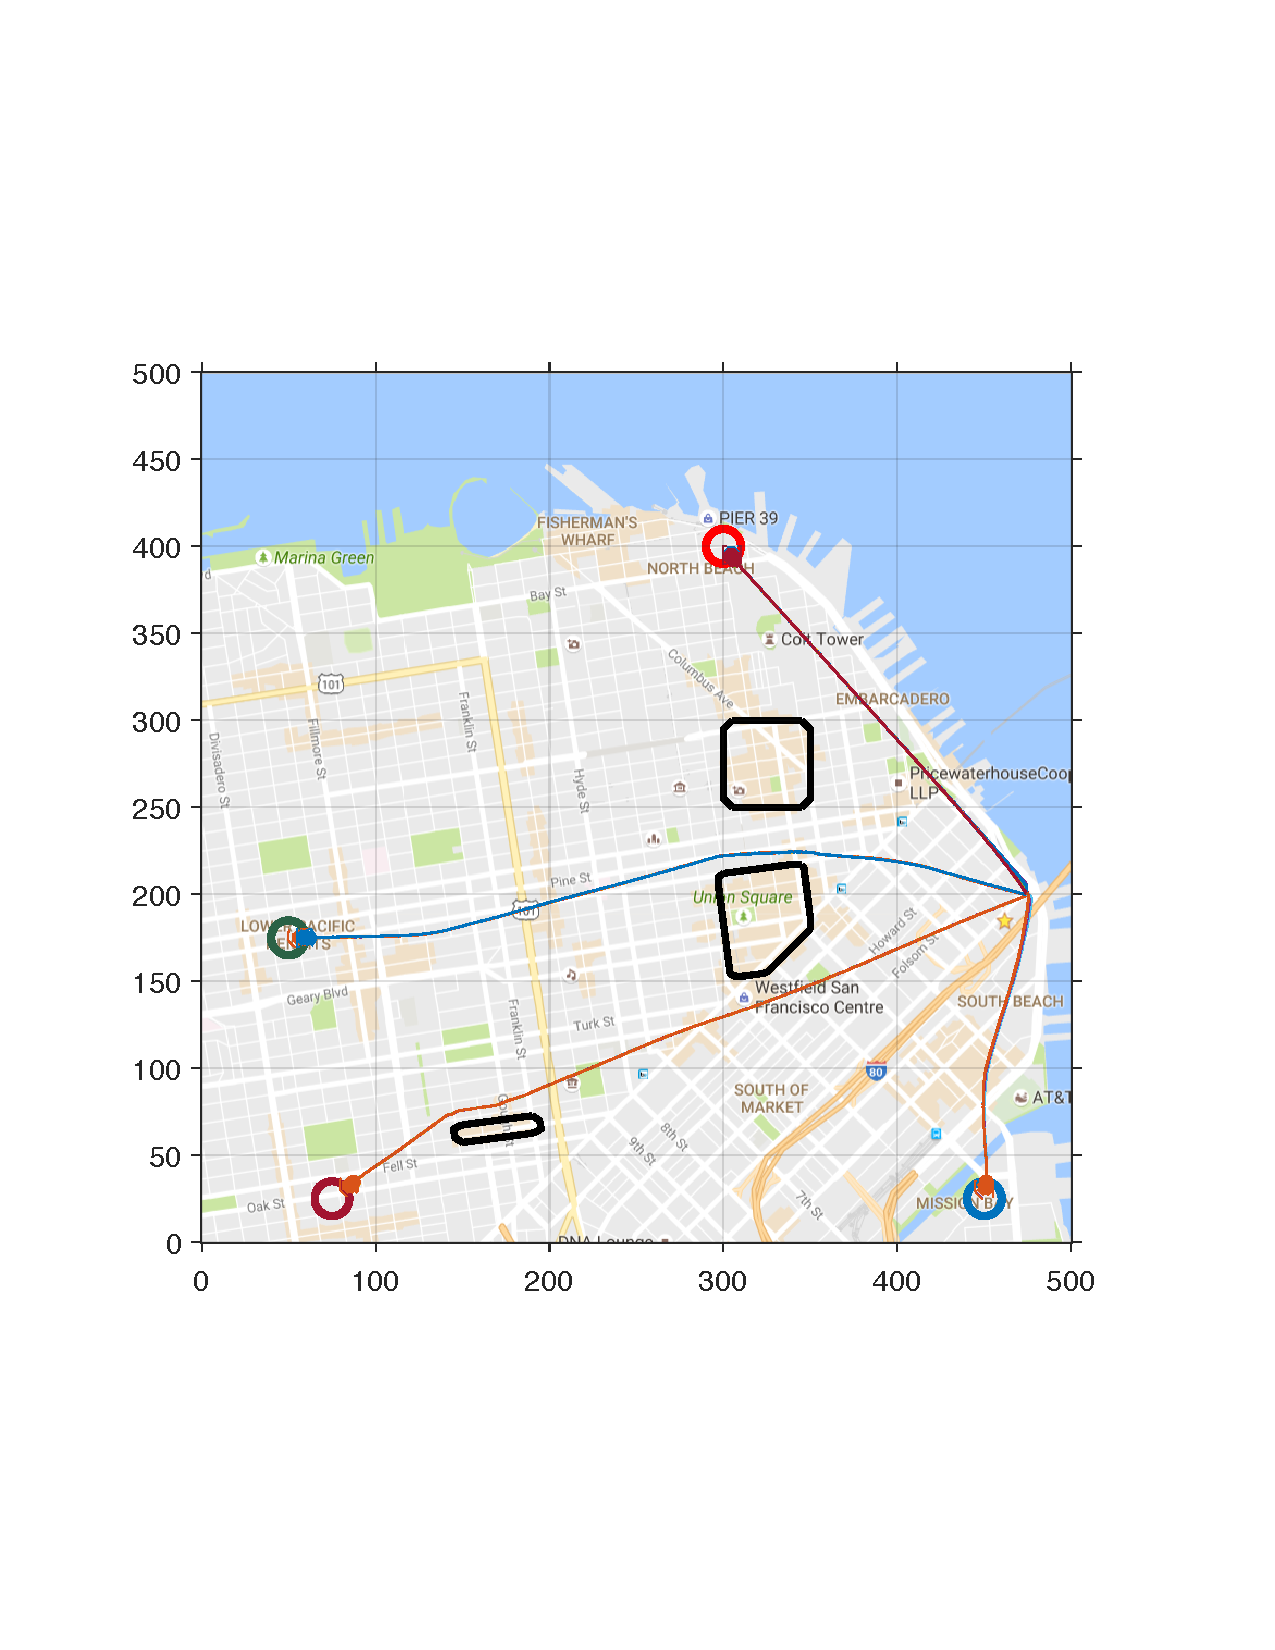
\includegraphics[width=\columnwidth]{figs/sf_d11sep10}
  \caption{Vehicle trajectories for Case-4: $d_r = 11$ m/s, $\sta_i = 10(i-1)$. Since different vehicles have different scheduled times of arrival, there is a single lane between every origin-destination pair.} 
  \label{fig:sf_d11sep10}
\end{figure}